如图,等边$\Delta$ABC的边长为3厘米,以点A为圆心、AC长为半径在三角形外画弧,交BA的延长线于点D;以点B为圆心、BD长为半径在三角形外画弧,交CB的延长线于点E;以点C为圆心、AC长为半径在三角形外画弧,交AC的延长线于点F,求最后所得图形CDEFC的周长.(结果保留$\pi$)

\begin{flushright}

    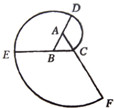
\includegraphics[height=2.86cm]{lib/image/MJA04020117.png}

\end{flushright}



